% !TEX root = MAIN.tex

\chapter{Data-driven Mutation Testing}
\label{chapter:datamutation}

% !TEX root = MutationTestingSurvey.tex

\section{Overview of the Data-driven Mutation Testing Process}
\label{sec:dataProcess}

	\begin{figure}
	\centering
		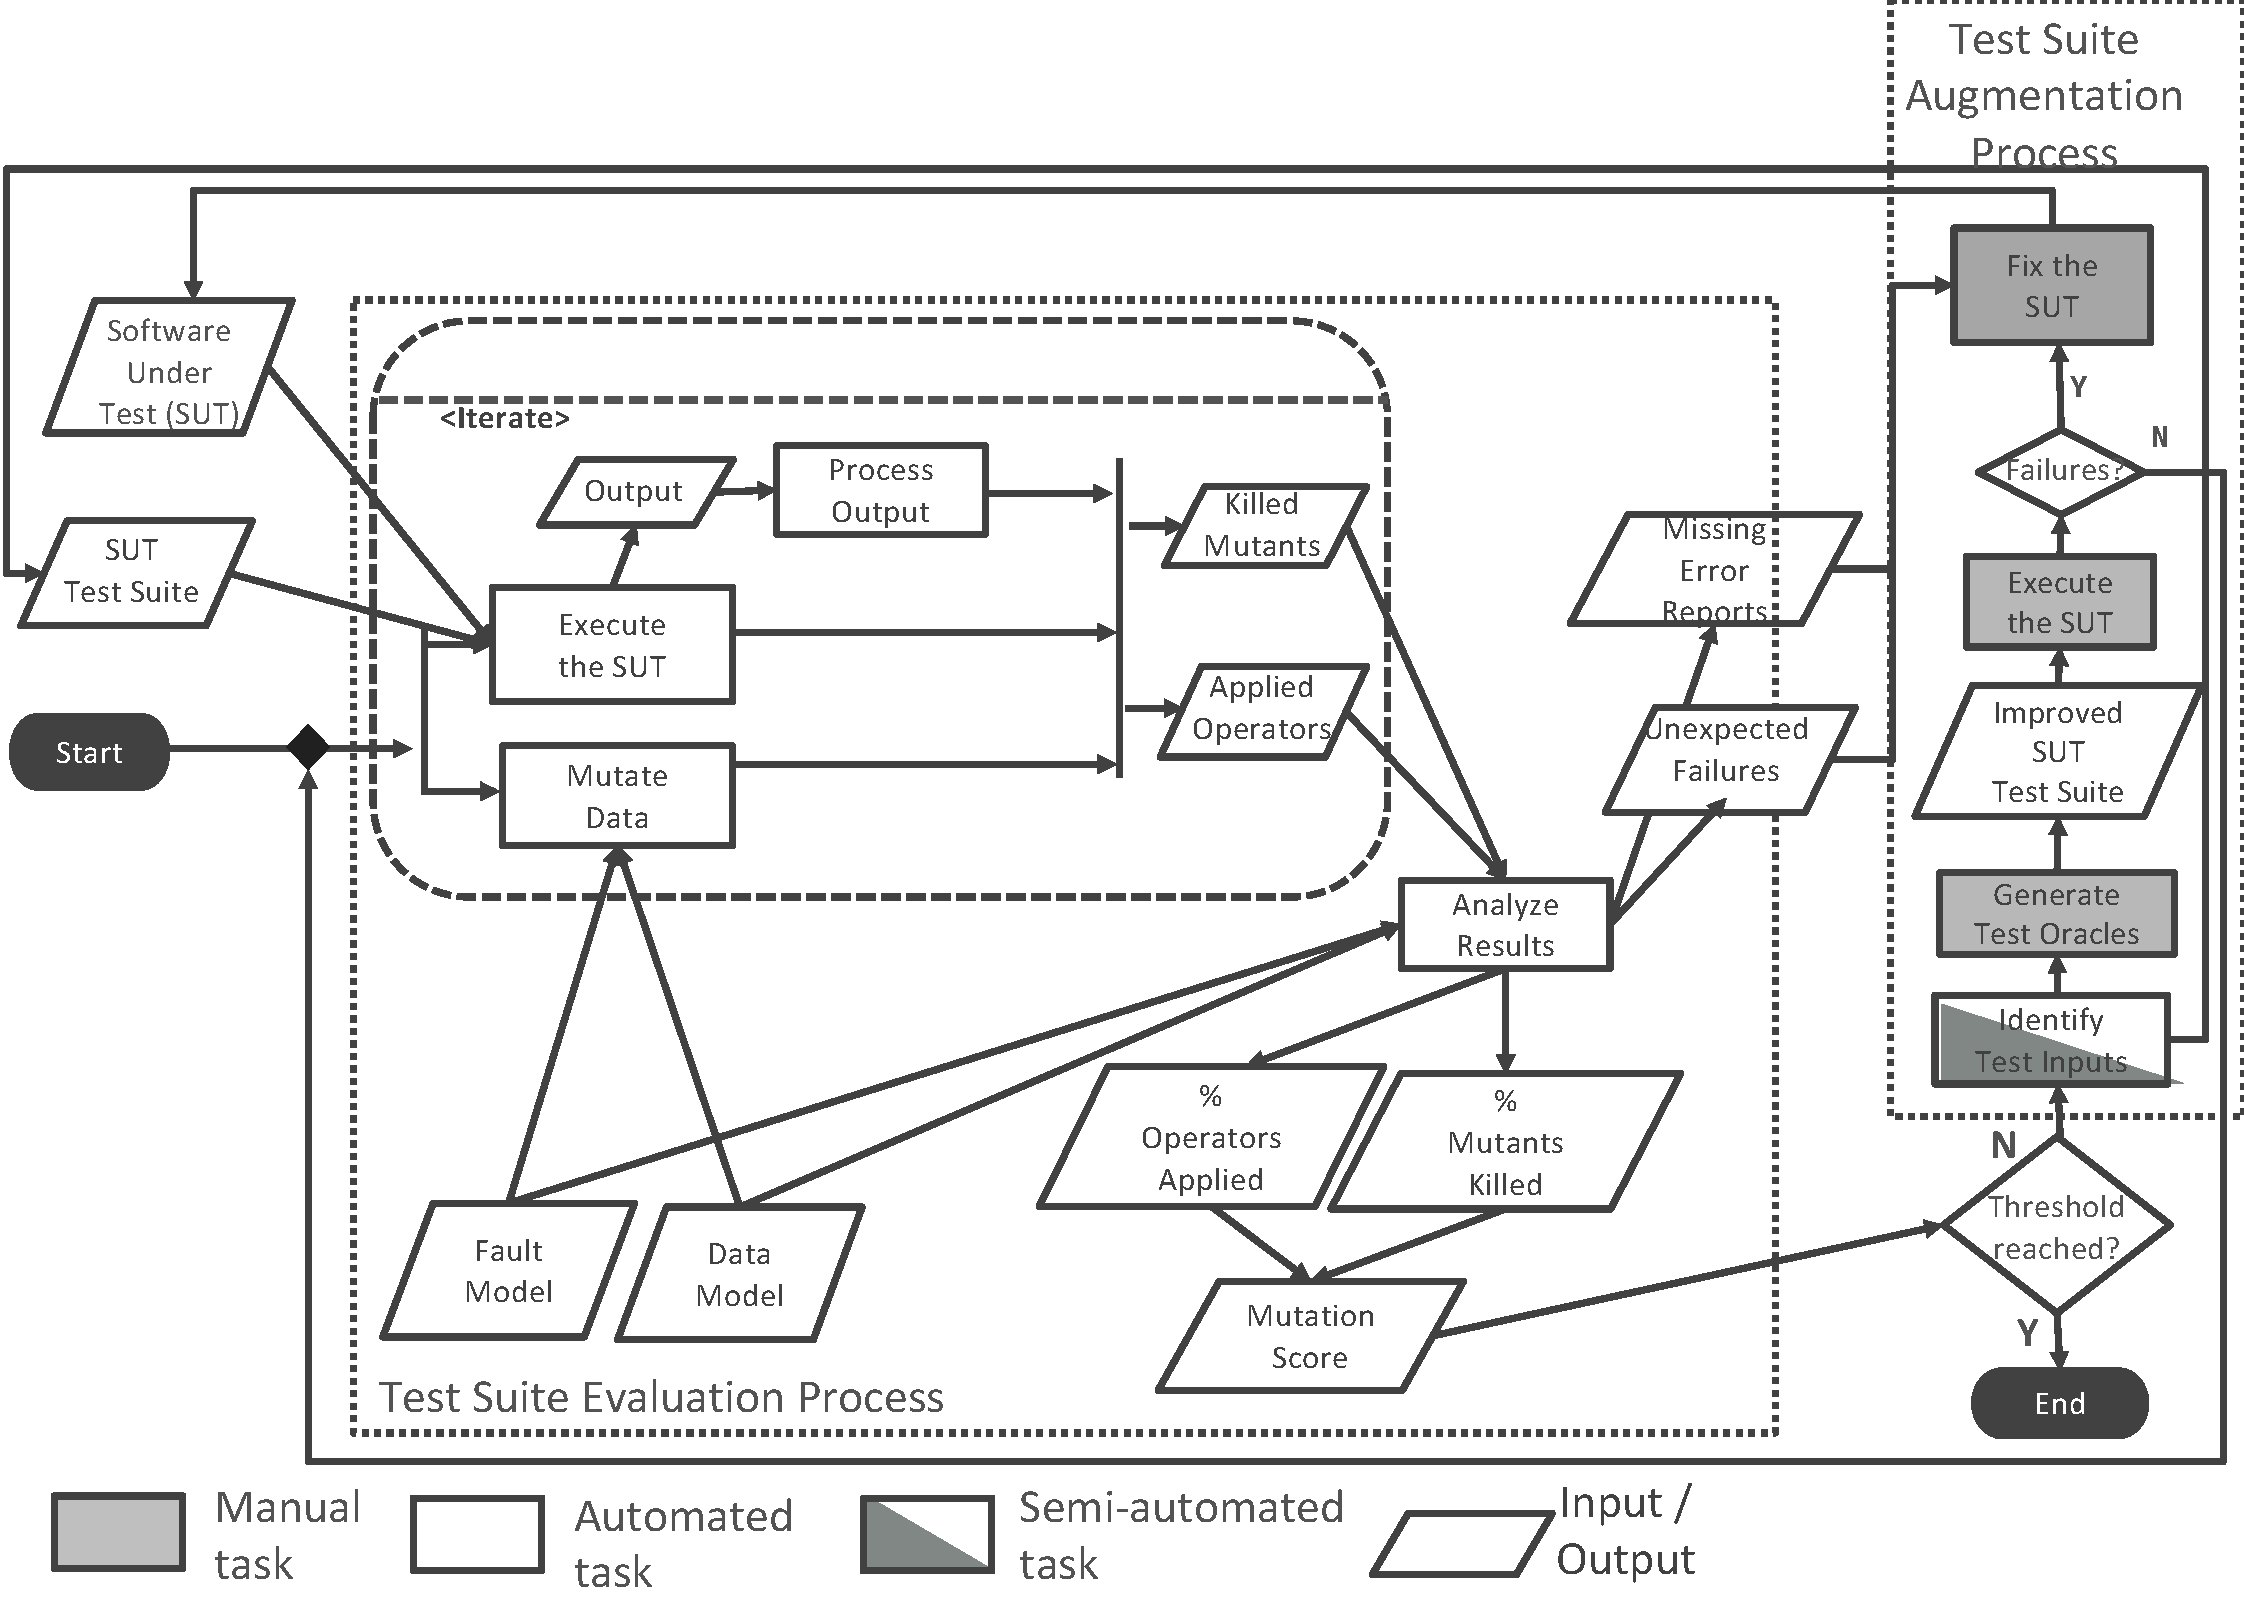
\includegraphics[width=\textwidth]{images/dataProcess}
		\caption{Data-driven Mutation Testing Process.}
		\label{fig:data:process}
	\end{figure}



This Chapter defines a test suite assessment process based on the injection of faults in the data processed by software components; we refer to this process as \INDEX{data-driven mutation testing}. 
%The definition of data-driven mutation testing is a unique contribution of this book; it has not been presented in previous literature work.

Data-driven mutation testing aims to assess test suites by simulating faults that affect the data produced, received, or exchanged by the software and its components.
It is based on a \INDEX{fault model} capturing the type of data faults that might affect the system. The fault model is produced by software engineers based on their domain knowledge and experience~\cite{di2015generating}. \MREVISION{C18}{The considered faults might be due to programming errors, hardware problems, or critical situations in the environment (e.g., noise in the channel).} The data is then automatically  mutated (i.e., modified) by a set of operators that aim to replicate the faults in the fault model. For example, the \INDEX{bit flip operator} flips a randomly selected bit of a field of the transmitted data (see Section~\ref{sec:faultModel}). 
%Mutation operators can be applied multiple times, on different data chunks or over repeated executions of a test case, ti


Figure \ref{fig:data:process} shows the reference data-driven mutation testing process that will be considered in FAQAS. The process is based on two main sub-processes, \EMPH{test suite evaluation} and \EMPH{test suite augmentation}, which are described in Sections~\ref{sec:data:test_suite_evaluation}~and~\ref{sec:data:test_suite_augmentation}, respectively. Differently from the code-driven mutation testing process introduced in Section~\ref{sec:process}, the data-driven mutation testing process has not been formalized by existing software testing literature. An extensive discussion of related work has been presented in deliverable D1.

Since data-driven mutation testing alters the data produced, received, or exchanged by the software or its components, it should be applied to evaluate test suites that trigger the execution and communication between multiple components (e.g., system or integration test cases). Data-driven mutation testing is not meant to be applied to assess unit test suites.

\clearpage
\section{Test Suite Evaluation} % (fold)
\label{sec:data:test_suite_evaluation}

The test suite evaluation process consists of three activities \EMPH{Execute the SUT}, \EMPH{Mutate Data},  and \EMPH{Analyze Results}.
The activity \INDEX{Execute the SUT} indicates that the SUT is executed against its automated test suite. 
The activity \INDEX{Mutate Data} concerns the automated modification of either the data received by the software, the data produced by the software, or the data exchanged by software components.
In Figure~\ref{fig:data:process}, the activity \EMPH{Mutate Data} is executed in parallel to the activity \EMPH{Execute the SUT} since data modification should occur at runtime during test cases execution, to simulate software faults affecting the data processed by the software.



%The fault model enables engineers to minimize the presence of equivalent mutants.
%The data model may capture the relation between inputs and outputs of the system

\begin{figure}
	\centering
		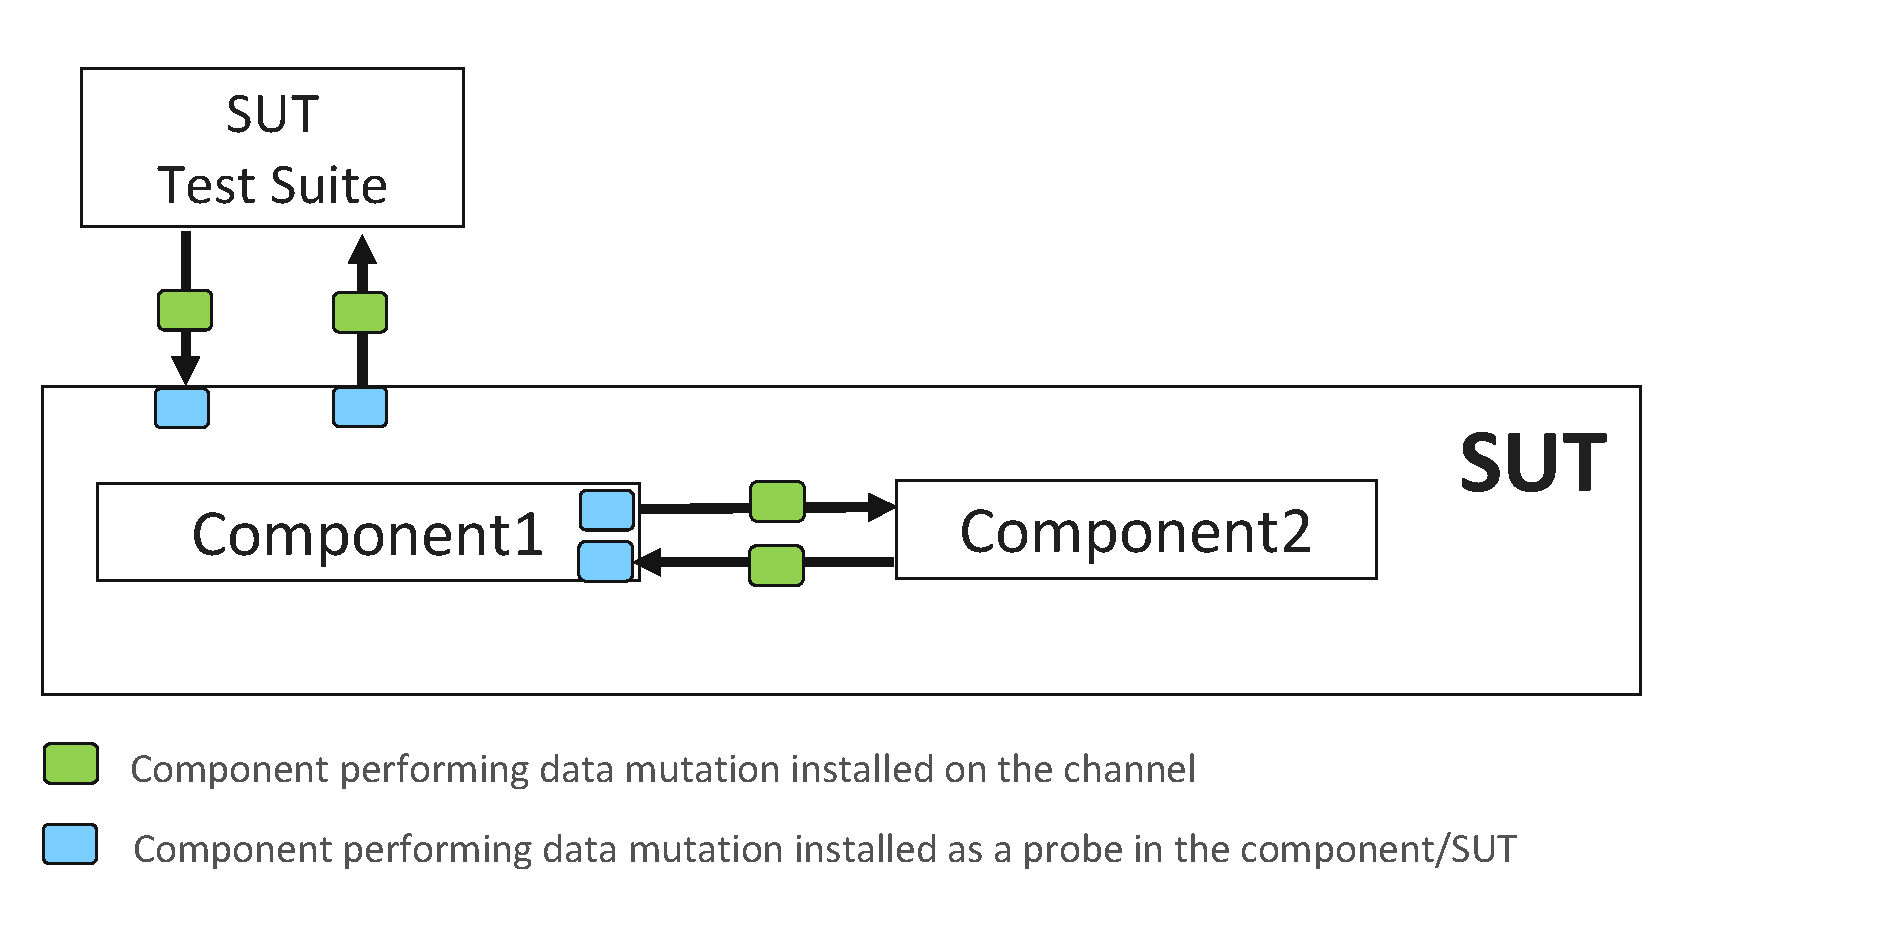
\includegraphics[width=10cm]{images/dataMutationExample}
		\caption{Example of implementation of a data mutation solution.}
		\label{fig:data:mutateData}
	\end{figure}
	
Figure~\ref{fig:data:mutateData} provides an example of how the Mutate Data activity can be implemented. Figure~\ref{fig:data:mutateData} shows that, to implement data mutation, it is necessary to integrate additional components that alter the data exchanged by the SUT components at runtime on a certain communication layer. We call such components \INDEX{mutation probes}.

An ideal target for data-driven mutation testing is the communication between loosely coupled software components; typically the ones that run on separated pieces of hardware (e.g., the on board controller and the ADCS).
In FAQAS case studies, the communication between such software components is performed by relying on APIs of a dedicated communication layer; which is typical in well designed software systems. The main functionality of such communication layer is to serialize and deserialize data that should be transmitted on the communication channel. In FAQAS case studies, the communication layer is either implemented in-house by the company that produced the case study or it is built by relying on the ASN.1 compiler architecture. In both the two cases, the communication layer implements distinct functions to serialize and deserialize data.
For this reason, in FAQAS, we expect mutation probes to be \EMPH{integrated into the software API functions that either serialize or deserialize the data being sent on the communication channel}.

In the case of a communication layer implemented in-house, we expect mutation probes to be integrated into the software under test by engineers who \EMPH{manually} add calls to the functions of a \INDEX{data-driven mutation testing API} in the source code of the software. Indeed, since communication APIs vary from system to system, it is not possible to define a tool that automatically modifies the source code or the executable code of the SUT.  Instead, we provide a \INDEX{data-driven mutation testing API} that implements the logic for mutating the data specified by the engineer.
To be applicable to a wide range of software systems, the API will provide methods that enable mutating data buffers provided as C arrays.
Figure~\ref{fig:data:mutationProbes} shows an example of a mutation probe manually integrated into the source code (API method names begin with the prefix \emph{\_FAQAS}).

In the case of a communication layer implemented by relying on the ASN.1 compiler, the FAQAS framework will automatically introduce mutation probes into the code that deserialize data.




\begin{figure}
	\centering
		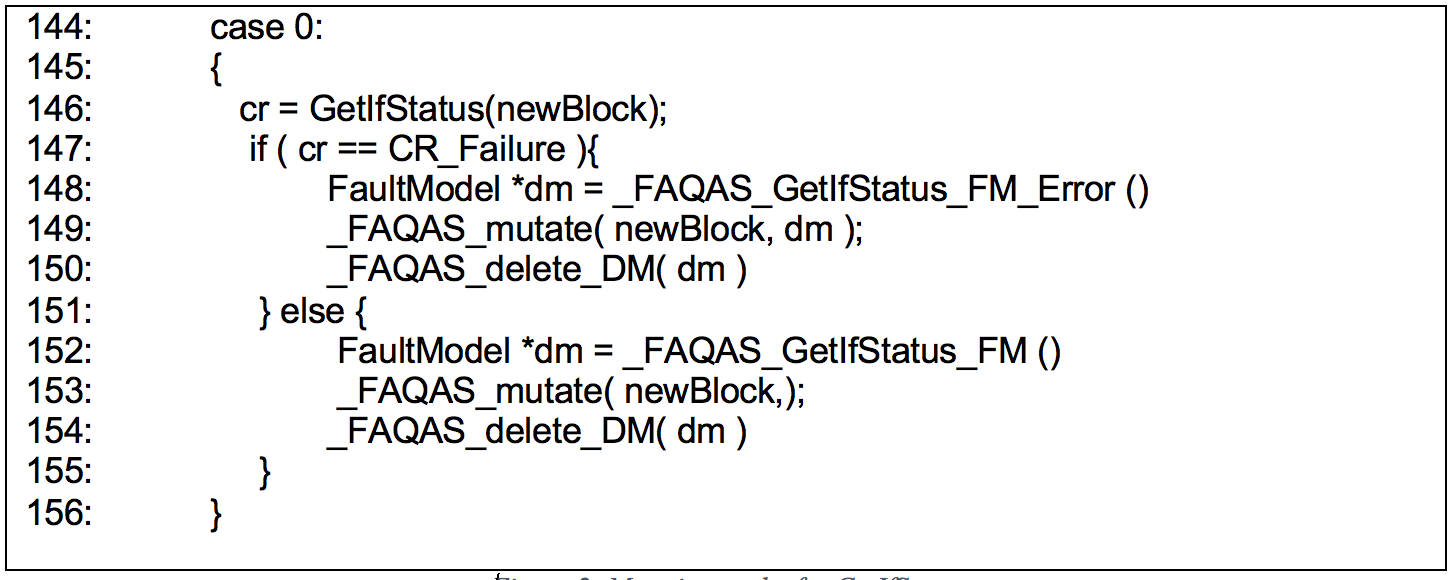
\includegraphics[width=10cm]{images/dataMutationProbes}
		\caption{Example of integration of data mutation probes.}
		\label{fig:data:mutationProbes}
	\end{figure}

%\TODO{ADD concrete example of integration}

	
%Data-driven mutation testing is driven by a faulty model specifying how to alter the data (i.e., the attributes declared in an ASN.1 grammar or the array items).	
In deliverable D1, we have clarified that, in a generic data-driven mutation testing process, the activity \EMPH{Mutate Data} may require a \INDEX{data model} that captures the characteristics and structure of the data to be mutated. 
The data model should be used to load a stream of bytes in structured form (e.g., an instance of a given data structure), which is necessary to drive data mutation. 
Also, the activity \EMPH{Mutate Data} should be driven by a \INDEX{fault model} that specifies the set of mutation operators to apply~\cite{di2015generating}. 
In FAQAS, the data model and the fault model are coupled into a same structured representation, i.e., the \INDEX{FAQAS fault model}, which is presented in Section~\ref{sec:faultModel}.


The activities \EMPH{Execute the SUT} and \EMPH{Mutate Data} are repeated till all the faults of the fault model had been applied. The possible stopping criteria are described in Section~\ref{sec:mutantsExecution}. 

The activity \INDEX{Process Outputs} processes all the outputs generated during the execution of test cases.
The collected outputs include the result of test cases execution (i.e., the list of test cases that either passed or failed) and the logs generated by the SUT during testing.
In the context of data-driven mutation testing both the \INDEX{test results} and the \INDEX{log files} are necessary to determine if a test suite kills a mutant.
Indeed, \emph{in the context of data-driven mutation testing a mutant is killed either if a test case fails, or if the software activates robustness features capable of handling the specific data fault.}
We need log files to determine if robustness features had been triggered.
For example, a system that implements a \INDEX{robust communication protocol} might simply request again the packets affected by errors thus avoiding failures. In this case, we need to inspect the log files to determine if the robustness feature had been triggered.
The fault model is expected to include only data fault classes that should either lead to failures or make the system generate an error entry in the log file.

Differently from code-driven mutation testing, data-driven mutation testing does not alter the software implementation but only the data processed by software components, for this reason it may help engineers to \INDEX{identify existing faults}, an objective that cannot be achieved by code-driven mutation testing. 
This is the case when \emph{Missing Error Reports} or \emph{Unexpected Failures }(e.g, crashes) are observed. In both the two cases, engineers should fix the system. In code-driven mutation testing, faults can be detected only after introducing new test cases that kill the generated mutants.

The activity \INDEX{Analyze Results} provides an assessment of the quality of the test suite for the SUT.
It is driven by two objectives:
\begin{itemize}
\item[(O1)] determine if the test suite is capable of detecting software faults that affect the data processed by the software components 
(e.g., we expect a test suite to fail in case the data exchanged by two components contains invalid values).
\item[(O2)] determine if the test suite exercises enough software behaviours to discover all the possible faults that may affect the data produced by the system
(i.e., it should be possible to alter the processed data to generate faulty data according to the fault model). 
\end{itemize}

\MREVISION{C19}{Objectives O1 and O2 are complementary, \REVTWO{C33}{they both should be addressed by data mutation.}
For example, a use case scenario for data-driven mutation testing could be the following: (i) data-driven mutation testing is applied to the data exchanged by \emph{component 1} and \emph{component 2} in Figure~\ref{fig:data:mutateData}, (ii) the data exchanged by the two components follow the data model in Figure~\ref{fig:DataDrivenSimpleExample}, and (iii) mutation testing is performed by applying the bit-flip mutation operator to every field of the messages being exchanged.
The data model in Figure~\ref{fig:DataDrivenSimpleExample} consists of a UML class diagram that indicates that the two components can send messages whose type can be either \emph{TimeMessage} or \emph{DataMessage}. A \emph{TimeMessage} contains only one field of type Long, which is the timestamp. 
A \emph{DataMessage} contains two fields, one field of type \emph{Integer} capturing the size of the payload, and one array of bytes containing the payload. 
Objective O1 is fulfilled when every mutant leads to the failure of least one test case.
Objective O2 is fulfilled when mutation testing generates at least (i) one \emph{TimeMessage} with field \emph{timestamp} being altered,
(ii) one \emph{DataMessage} with field \emph{size} being altered,
and (iii) one \emph{DataMessage} with field \emph{payload} being altered.
For a test suite consisting of two test cases that trigger the exchange of the messages as in the bottom-left part of Figure~\ref{fig:DataDrivenSimpleExample}, the execution of the bit flip mutation operator may lead to messages that lead to test failures. Since all the mutants are killed (i.e., the two test cases fail), objective O1 is achieved. However, the test suite does not lead to the exchange of any message of type \emph{DataMessage}, for this reason objective O2 is not achieved. Objective O2 enables us to determine that the test suite does not exercise the case in which the two components exchange messages of type \emph{DataMessage}. When data-driven mutation testing is performed against components that are expected to guarantee robustness against the exchange of erroneous data, as a by-product, objective O2 also ensures that components' robustness is properly tested.}



\REVTWO{C34}{Activity \emph{Analyze Results} concerns the automated computation of the \INDEX{mutation score} from execution data. It is 
computed as the weighted average of the percentage of mutants being killed and the percentage of mutation operators applied.}
The former enables data-driven mutation to achieve objective O1 in Section~\ref{sec:dataProcess}, the latter objective O2. 
%Details are provided in Section~\ref{sec:data:mutationscore}.

\REVTWO{C34}{Activity \emph{Analyze Results} takes as input the the data model, the fault model, the list of killed mutants, and the list of mutation operators applied.}
The list of applied mutation operators should enable engineers to determine if all the available mutation operators have been applied.


\begin{figure}[t!]
  \centering
    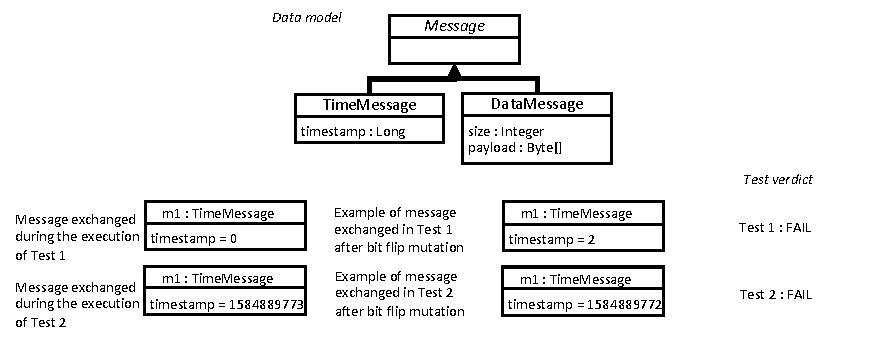
\includegraphics{images/DataDrivenSimpleExample}
      \caption{Simplified data mutation example.}
      \label{fig:DataDrivenSimpleExample}
\end{figure}

\clearpage



\clearpage
\subsection{FAQAS Fault Model}
\label{sec:dataModel}
\label{sec:faultModel}





A building block of the fault model are a set of \EMPH{data fault classes}.
A  \INDEX{data fault class} captures the type of an error that might affect the data. In turns, it specifies the mutation that should be applied in order to replace valid data with erroneous data. For each fault class we have defined a corresponding \INDEX{data mutation operator} having the same name. 
Each {data mutation operator} performs data mutation by applying a \INDEX{data mutation operation} (e.g., set a value above the upper range value). Mutation operators might apply one or more data mutation operations.
Each data mutation operator can be configured with a set of parameters. 

Table~\ref{table:faultModel:FAQAS} provides the list of data fault classes supported by FAQAS along with a description. For each fault class we indicate the data types to which it is expected to be applied, we identify four data types: 
\begin{itemize}
\item int, which indicates an integer
\item float, which indicates a floating point number
\item double, which indicates a double precision floating point number
\item bin, which indicate data that should be treated in its binary form
\end{itemize}


In FAQAS, data-driven mutation testing is performed by modifying either data that is stored in an array or in a data structure defined through the ASN.1 grammar. The following subsections describe the two distinct cases.







% !TEX root = ../MAIN.tex
\begin{table}[h]
\begin{center}
\scriptsize
\begin{tabular}{|p{2cm}|p{2cm}|p{4cm}|p{6cm}|}
\hline
\textbf{Fault Class}&\textbf{Types}&\textbf{Parameters}&\textbf{Description}\\
\hline
Value above threshold (VAT)&
\begin{minipage}{6cm}
INT\\
LONG INT\\
FLOAT\\
DOUBLE
\end{minipage}
&
\begin{minipage}{6cm}
T: threshold\\
D: delta with respect to threshold\\
\end{minipage}
&
\begin{minipage}{6cm}
The value is above a threshold T for a delta D. 

\EMPH{Data mutation operation:} The mutation is performed by replacing the current value (a number) with a value of the same type that is equal to $(T+D)$.
\end{minipage}
\\

\hline
Value below threshold (VBT)&
\begin{minipage}{6cm}
INT\\
LONG INT\\
FLOAT\\
DOUBLE
\end{minipage}
&
\begin{minipage}{6cm}
T: threshold\\
D: delta with respect to threshold\\
\end{minipage}
&
\begin{minipage}{6cm}
The value is below a threshold T for a delta D. 

\EMPH{Data mutation operation:} The mutation is performed by replacing the current value (a number) with a value of the same type that is equal to $(T-D)$.
\end{minipage}
\\



\hline
Value out of range (VOR)&
\begin{minipage}{4cm}
INT\\
LONG INT\\
FLOAT\\
DOUBLE
\end{minipage}
&
\begin{minipage}{4cm}
MIN: minimum valid value\\
MAX: maximum valid value\\
D: delta with respect to minimum/maximum valid value
\end{minipage}
&
\begin{minipage}{6cm}
The value is out of the valid range MIN-MAX. 

\EMPH{Data mutation operations (2):}  The mutation is performed by replacing the current value (a number) with 
\begin{itemize}
\item a value of the same type that is equal to $(MIN-D)$
\item a value of the same type that is equal to $(MAX+D)$
\end{itemize}
\end{minipage}
\\

\hline
Bit flip (BF)&
BIN
&
\begin{minipage}{4cm}
MIN: lower bit\\
MAX: higher bit\\
STATE: mutate only if the bit is in the given state\\
\TRFOUR{VALUE: integer specifying the number of bits to mutate}\\
\end{minipage}
&
\begin{minipage}{6cm}
A number of bits randomly chosen in the positions between MIN and MAX (included) are flipped.

\EMPH{Data mutation operation:} the operator flips N randomly selected bit.
If STATE is specified, the mutation is applied only if  the bit is in the specified state. Parameter VALUE specifies the number of bits to mutate.
\end{minipage}
\\

\hline
Invalid numeric value (INV)&
\begin{minipage}{6cm}
INT\\
LONG INT\\
FLOAT\\
DOUBLE
\end{minipage}
&
\begin{minipage}{4cm}
MIN: lower valid value\\
MAX: higher valid value\\
\TRFOUR{D: distribution to follow}\\
\TRFOUR{VALUE: mean value for normal distribution}\\
\end{minipage}
&
\begin{minipage}{6cm}
The value is legal (i.e., in the specified range) but different than the current one, which, in this case, is expected to be consistent with the status of the system.

\EMPH{Data mutation operation:} Mutation is performed by replacing the current value with a different value randomly sampled in the specified range. The parameter D specified the distribution to follow when performing the mutation\footnote{In our implementation 0 indicates uniform, 1 indicates normal around the specified value (but in range).}
\end{minipage}
\\

\hline
Illegal Value (IV)
&
\begin{minipage}{6cm}
INT\\
LONG INT\\
FLOAT\\
DOUBLE
\end{minipage}
&
\begin{minipage}{6cm}
VALUE: illegal value that is observed\\
\end{minipage}
&
\begin{minipage}{6cm}
The value is illegal and equal to the provided one (i.e., parameter \emph{VALUE}).

\EMPH{Data mutation operation:} Mutation is performed by replacing the current value with the value \emph{VALUE}, if different than the current one.
\end{minipage}
\\

\hline
\TRFOUR{Anomalous Signal Amplitude (ASA)}
&
\begin{minipage}{6cm}
INT\\
LONG INT\\
FLOAT\\
DOUBLE
\end{minipage}
&
\begin{minipage}{6cm}
T: change point\\
D: delta to add/remove\\
V: value to multiply\\
\end{minipage}
&
\begin{minipage}{6cm}
The value is modified by amplifying/reducing it by a factor V and adding or removing D from the observed value. It is used to "amplify" a signal in a constant manner to simulate unusual signal. T indicates the observed value below which instead of adding  we subtract .

\EMPH{Data mutation operation:} Mutation is performed by replacing the current value ($v$) with the value ($v'$) computed as follows:

\[
v' =  
    \begin{cases}
      T+(  (v-T)*V  ) + D   & \mathit{if}\ v \ge T\\
      T - (  (T-v)*V  ) - D   & \mathit{if}\ v < T
    \end{cases}       
\]
\end{minipage}
\\


\hline
\TRFOUR{Signal Shift (SS)}
&
\begin{minipage}{6cm}
INT\\
LONG INT\\
FLOAT\\
DOUBLE
\end{minipage}
&
\begin{minipage}{6cm}
D: delta by which the signal should be shifted\\
\end{minipage}
&
\begin{minipage}{6cm}
The value is modified by adding a value D. It simulate an anomalous shift in the signal.
\end{minipage}
\\





\hline
\TRFOUR{Hold Value (HV)}
&
\begin{minipage}{6cm}
BIN\\
INT\\
LONG INT\\
FLOAT\\
DOUBLE
\end{minipage}
&
\begin{minipage}{6cm}
V: number of times to repeat the same value\\
\end{minipage}
&
\begin{minipage}{6cm}
This operator keeps repeating an observed value for $V$ times. It emulates a constant signal replacing a signal supposed to vary.
\end{minipage}
\\



\hline
\TRFOUR{Array Swap (AS)}
&
\begin{minipage}{6cm}
ARRAY\_*\\
\end{minipage}
&
\begin{minipage}{6cm}
MIN: position of element A\\
MAX: position of element B\\
VALUE: number of elements to move\\
\end{minipage}
&
\begin{minipage}{6cm}
Replace a number of elements (number specified by VALUE) located starting from position MIN, with a number of elements located starting from position MAX, and viceversa.
\EMPH{Data mutation operation:} Mutation is performed by replacing the two set of elements with each other.
\end{minipage}
\\


\hline
\TRFOUR{Array Random Swap (ARS)}
&
\begin{minipage}{6cm}
ARRAY\_*\\
\end{minipage}
&
\begin{minipage}{6cm}
MIN: min position of element A/B\\
MAX: max position of element A/B\\
VALUE: number of elements to move\\
\end{minipage}
&
\begin{minipage}{6cm}
Replace a number of elements (number specified by VALUE) located in a position between MIN and MAX, with a number of elements located in a position between MIN and MAX. MIN and MAX specify a position with respect to the beginning and end of the array.  For example, MIN=0 indicates the first element of teh array, MIN=-2 indicates the second element of the array.
\EMPH{Data mutation operation:} Mutation is performed by replacing the two set of elements with each other.
\end{minipage}
\\



%Incorrect Identifier& Several transmission data fields have fixed values, for example fields identifying the transmitting satellite. Hardware/software errors may assign incorrect identifiers.\\
%%Incorrect Checksum& Hardware/software errors may result in an incorrect checksum for a Packet or VCDU.\\
%Incorrect Counter& Counters are used to track Packet or VCDU ordering. Hardware/software errors may assign incorrect counter values.\\
%Flipped Data Bits& Physical channel noise may flip one or more bits in the data transmission.\\
\hline
\end{tabular}
\end{center}
\caption{Data Fault Classes}
\label{table:faultModel:FAQAS}
\end{table}%

\subsubsection{Fault Model Specifications for Data Buffers}

When the data to be mutated is stored in an array, we require the definition of a fault model in the form of a block diagram since this format enables to represent the sequence of data items in the array. 
For each data block the FAQAS fault model captures its type and a list of data fault classes that might affect the block. 
The type of the data block indicates how the values of bits should be interpreted (e.g., as a floating point number). Since a data type may span over multiple items of the data buffer, for each block, we may indicate whether also the values of the following blocks should be used to load the data.

Table~\ref{table:faultModel:example} provides an example of two fault models described in tabular form. 
It resembles the CSV format supported by the FAQAS toolset. For each data item we report the span, type, and fault class. For each fault class we indicate the values of the configuration parameters for the corresponding mutation operator.


% !TEX root = ../MAIN.tex
\begin{table}[h]
\begin{center}
\small
\begin{tabular}{|p{1cm}|p{2cm}|p{1cm}|p{1cm}|p{1cm}|p{1cm}|p{1cm}|p{2cm}|p{1cm}|p{1cm}|}
\hline
\textbf{Fault Model Name}&\textbf{DataItem}&\textbf{Span}&\textbf{Type}&\textbf{Fault Class}&\textbf{Min}&\textbf{Max}&\textbf{Threshold}&\textbf{Delta}&\textbf{State}\\
\hline
IfHK&0&1&BIN&BF&0&0&-&-&-\\
IfHK&1&1&INT&VOR&0&5&-&1&-\\
IfHK&2&2&BIN&BF&0&63&-&-&-\\
IfHK&4&1&BIN&BF&0&0&-&-&-\\
\hline
IfStatus&0&1&BIN&BF&0&0&-&-&-\\
\hline
\end{tabular}
\end{center}
\caption{Driven Fault Model Buffer}
\label{table:faultModel:example}
\end{table}%

\clearpage
\subsubsection{Fault Model Specifications for ASN.1 grammar}

The ASN.1 grammar enables engineers to specify data structures where the types of the items in the data structure are selected from a predefined set.

%When the data to be mutated is stored in a data structure defined through the ASN.1 grammar, the fault model is specified by indicating which operators to apply on the specific fields of the data structure. 

We have identified a set of feasible fault classes for each type supported by the ASN1CC compiler.
The corresponding mutation operators are automatically configured based on the ASN.1 grammar (e.g., in the case of an attribute of type INTEGER, the min/max values of the VOR operator are derived from the boundaries of the INTEGER type).
Table~\ref{table:faultModel:FAQAS:ASN1} provides, for each of such types, the feasible fault classes and the configurations for the mutation operators.
In the configuration for the mutation operators, we refer to the variables (e.g., MIN and MAX) appearing in the ASN.1 xml file.

Figure~\ref{fig:ASN1ProbesGeneration} provides an overview of the process in place to generate probes including the fault model.
The engineer first export the ASN.1 grammar as XML, then he modifies the generated file by specifying, for each \emph{Asn1Type}, the mutation operator to be used (this is done by adding an xml attribute called \emph{MutationOperator} with a value specifying the name of the operator). 

An example is provided in Listings~\ref{asnXML} and \ref{asnXMLUpdated}. Listing~\ref{asnXML} provides the xml generated by the grammar, which includes two INTEGER types.
Listing~\ref{asnXMLUpdated} provides the xml updated by the engineer, who indicates that the two integers should be mutated with the VAR and the VOR operator. To tune the operators, the engineer updates the MIN and MAX values for those integers to capture only nominal values. 
In the case of the first integer (the one to be mutated with VAR), the engineer sets 5 as MAX.
In the case of the second integer (the one to be mutated with VOR), the engineer sets MIN and MAX to 0 and 50 respectively.
%The engineer can tune the mutation by changing the value ranges associated to the different types. For example, this could be done to restrict the valid range of an INTEGER from (MIN=-100, MAX=100) to a nominal range of (MIN=0,MAX=50).
In case a data type is defined through value range constraints, the FAQAS framework will configure one mutation operator instance for each range.

% !TEX root = ../MAIN.tex
\begin{table}[h]
\begin{center}
\small
\begin{tabular}{|p{2cm}|p{2cm}|p{4cm}|p{4cm}|}
\hline
\textbf{Types}&\textbf{Fault Classes}&\textbf{Parameters}&\textbf{Description}\\
\hline
INTEGER&
VAT&
\begin{minipage}{4cm}
T: MAX\\
D: 1\\
\end{minipage}
&
\begin{minipage}{4cm}
\end{minipage}
\\
\hline
INTEGER&
VBT&
\begin{minipage}{4cm}
T: MIN\\
D: 1\\
\end{minipage}
&
\begin{minipage}{4cm}
\end{minipage}
\\
\hline
INTEGER&
VOR&
\begin{minipage}{4cm}
MIN: MIN\\
MAX: MAX\\
D: 1\\
\end{minipage}
&
\begin{minipage}{4cm}
\end{minipage}
\\
\hline
REAL&
VAT&
\begin{minipage}{4cm}
T: MAX\\
D: 1\\
\end{minipage}
&
\begin{minipage}{4cm}
\end{minipage}
\\
\hline
REAL&
VBT&
\begin{minipage}{4cm}
T: MIN\\
D: 1\\
\end{minipage}
&
\begin{minipage}{4cm}
\end{minipage}
\\
\hline
REAL&
VOR&
\begin{minipage}{4cm}
MIN: MIN\\
MAX: MAX\\
D: 1\\
\end{minipage}
&
\begin{minipage}{4cm}
\end{minipage}
\\
\hline
ENUMERATED&
INV&
\begin{minipage}{4cm}
MIN: MIN\\
MAX: MAX\\
D: 1\\
\end{minipage}
&
\begin{minipage}{4cm}
\end{minipage}
\\
\hline
BOOLEAN&
BF&
\begin{minipage}{4cm}
MIN: 0\\
MAX: 0\\
\end{minipage}
&
\begin{minipage}{4cm}
\end{minipage}
\\
\hline
NULL&
BF&
\begin{minipage}{4cm}
MIN: 0\\
MAX: 0\\
\end{minipage}
&
\begin{minipage}{4cm}
\end{minipage}
\\
\hline
BIT STRING&
BF&
\begin{minipage}{4cm}
MIN: 0\\
MAX: 0\\
\end{minipage}
&
\begin{minipage}{4cm}
\end{minipage}
\\
\hline
OCTET STRING&
BF&
\begin{minipage}{4cm}
MIN: 0\\
MAX: 0\\
\end{minipage}
&
\begin{minipage}{4cm}
\end{minipage}
\\
\hline
IA5STRING&
BF&
\begin{minipage}{4cm}
MIN: 0\\
MAX: 0\\
\end{minipage}
&
\begin{minipage}{4cm}
\end{minipage}
\\
\hline
NUMERIC STRING&
BF&
\begin{minipage}{4cm}
MIN: 0\\
MAX: 0\\
\end{minipage}
&
\begin{minipage}{4cm}
\end{minipage}
\\
\hline
SEQUENCE&
-&
\begin{minipage}{4cm}
\end{minipage}
&
\begin{minipage}{4cm}
No mutation environed for this type.
\end{minipage}
\\
\hline
SET&
-&
\begin{minipage}{4cm}
\end{minipage}
&
\begin{minipage}{4cm}
No mutation environed for this type.
\end{minipage}
\\
\hline
CHOICE&
-&
\begin{minipage}{4cm}
\end{minipage}
&
\begin{minipage}{4cm}
No mutation environed for this type.
\end{minipage}
\\
\hline
SEQUENCE OF&
-&
\begin{minipage}{4cm}
\end{minipage}
&
\begin{minipage}{4cm}
No mutation environed for this type.
\end{minipage}
\\
\hline
SET OF&
-&
\begin{minipage}{4cm}
\end{minipage}
&
\begin{minipage}{4cm}
No mutation environed for this type.
\end{minipage}
\\



%Incorrect Identifier& Several transmission data fields have fixed values, for example fields identifying the transmitting satellite. Hardware/software errors may assign incorrect identifiers.\\
%%Incorrect Checksum& Hardware/software errors may result in an incorrect checksum for a Packet or VCDU.\\
%Incorrect Counter& Counters are used to track Packet or VCDU ordering. Hardware/software errors may assign incorrect counter values.\\
%Flipped Data Bits& Physical channel noise may flip one or more bits in the data transmission.\\
\hline
\end{tabular}
\end{center}
\caption{Data Fault Classes for ASN.1 data types.}
\label{table:faultModel:FAQAS:ASN1}
\end{table}%



\begin{figure}[tb]
  \centering
    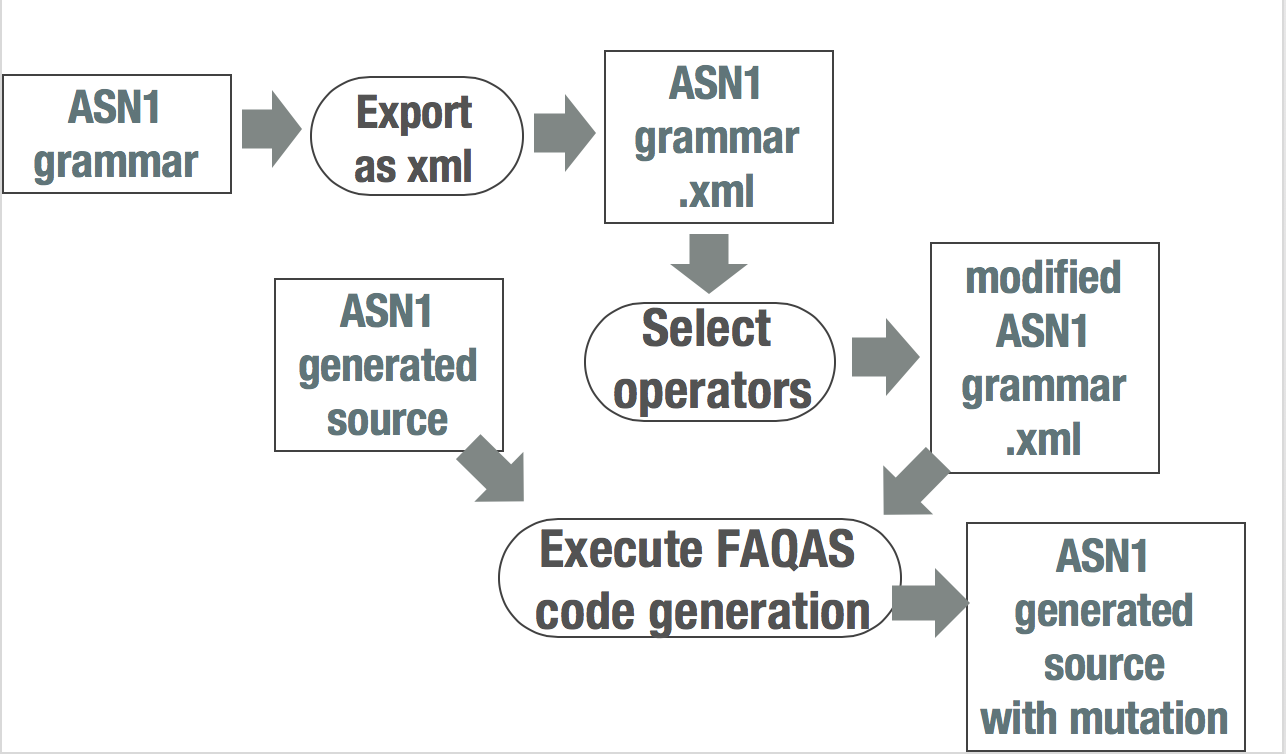
\includegraphics[width=12cm]{images/ASN1mutationProces}
      \caption{Data-driven probes generation process for ASN1.}
      \label{fig:ASN1ProbesGeneration}
\end{figure}


% !TEX root =  ../MAIN.tex

\begin{minipage}{15cm}
\begin{lstlisting}[style=CStyle, caption=Portion of an XML ASN1 grammar., label=asnXML, mathescape=true]
<TypeAssignment Name="TypeNested" CName="TypeNested" AdaName="TypeNested" Line="16" CharPositionInLine="0">
            <Asn1Type id="MY-MODULE.TypeNested" Line="16" CharPositionInLine="15" ParameterizedTypeInstance="false">
              <SEQUENCE acnMaxSizeInBits="3087" acnMinSizeInBits="2688" uperMaxSizeInBits="3087" uperMinSizeInBits="528">
                <SEQUENCE_COMPONENT Name="intVal" Line="17" CharPositionInLine="4" AdaName="intVal" CName="intVal">
                  <Asn1Type id="MY-MODULE.TypeNested.intVal" Line="17" CharPositionInLine="11" ParameterizedTypeInstance="false">
                    <INTEGER acnMaxSizeInBits="4" acnMinSizeInBits="4" uperMaxSizeInBits="4" uperMinSizeInBits="4">
                      <Constraints>
                        <Range>
                          <Min>
                            <IntegerValue>0</IntegerValue>
                          </Min>
                          <Max>
                            <IntegerValue>10</IntegerValue>
                          </Max>
                        </Range>
                      </Constraints>
                      <WithComponentConstraints />
                    </INTEGER>
                  </Asn1Type>
                </SEQUENCE_COMPONENT>
                <SEQUENCE_COMPONENT Name="int2Val" Line="18" CharPositionInLine="4" AdaName="int2Val" CName="int2Val">
                  <Asn1Type id="MY-MODULE.TypeNested.int2Val" Line="18" CharPositionInLine="12" ParameterizedTypeInstance="false">
                    <INTEGER acnMaxSizeInBits="5" acnMinSizeInBits="5" uperMaxSizeInBits="5" uperMinSizeInBits="5">
                      <Constraints>
                        <Range>
                          <Min>
                            <IntegerValue>-100</IntegerValue>
                          </Min>
                          <Max>
                            <IntegerValue>100</IntegerValue>
                          </Max>
                        </Range>
                      </Constraints>
                      <WithComponentConstraints />
                    </INTEGER>
                  </Asn1Type>
                </SEQUENCE_COMPONENT>
\end{lstlisting}
\end{minipage}


% !TEX root =  ../MAIN.tex

\begin{minipage}{15cm}
\begin{lstlisting}[style=CStyle, caption=Portion of an XML ASN1 grammar., label=asnXMLUpdated, mathescape=true]
<TypeAssignment Name="TypeNested" CName="TypeNested" AdaName="TypeNested" Line="16" CharPositionInLine="0">
            <Asn1Type id="MY-MODULE.TypeNested" Line="16" CharPositionInLine="15" ParameterizedTypeInstance="false">
              <SEQUENCE acnMaxSizeInBits="3087" acnMinSizeInBits="2688" uperMaxSizeInBits="3087" uperMinSizeInBits="528">
                <SEQUENCE_COMPONENT Name="intVal" Line="17" CharPositionInLine="4" AdaName="intVal" CName="intVal">
                  <Asn1Type id="MY-MODULE.TypeNested.intVal" Line="17" CharPositionInLine="11" ParameterizedTypeInstance="false">
                    <INTEGER MutationOperator="VAT" acnMaxSizeInBits="4" acnMinSizeInBits="4" uperMaxSizeInBits="4" uperMinSizeInBits="4">
                      <Constraints>
                        <Range>
                          <Min>
                            <IntegerValue>0</IntegerValue>
                          </Min>
                          <Max>
                            <IntegerValue>5</IntegerValue>
                          </Max>
                        </Range>
                      </Constraints>
                      <WithComponentConstraints />
                    </INTEGER>
                  </Asn1Type>
                </SEQUENCE_COMPONENT>
                <SEQUENCE_COMPONENT Name="int2Val" Line="18" CharPositionInLine="4" AdaName="int2Val" CName="int2Val">
                  <Asn1Type id="MY-MODULE.TypeNested.int2Val" Line="18" CharPositionInLine="12" ParameterizedTypeInstance="false">
                    <INTEGER MutationOperator="VOR" acnMaxSizeInBits="5" acnMinSizeInBits="5" uperMaxSizeInBits="5" uperMinSizeInBits="5">
                      <Constraints>
                        <Range>
                          <Min>
                            <IntegerValue>0</IntegerValue>
                          </Min>
                          <Max>
                            <IntegerValue>50</IntegerValue>
                          </Max>
                        </Range>
                      </Constraints>
                      <WithComponentConstraints />
                    </INTEGER>
                  </Asn1Type>
                </SEQUENCE_COMPONENT>
\end{lstlisting}
\end{minipage}






\clearpage
\subsection{FAQAS Data Mutation API and Probes}
\label{sec:FAQASDataMutationProbes}

In FAQAS, the data-driven mutation testing API is automatically generated from the fault model provided by engineers. Data mutation probes are either manually implemented by software engineers (in the case data mutation should target an ad-hoc communication layer that works with data buffers) or automatically generated by the toolset (in the case data mutation should target an ASN.1-based communication layer).

Section~\ref{sec:FAQASDataMutationProbesBuffer} describes the case of data buffers (i.e., C arrays).
Section~\ref{sec:FAQASDataMutationProbesASN} describes the case of ASN.1.


\subsubsection{Data Mutation for Data Buffers}
\label{sec:FAQASDataMutationProbesBuffer}

Figure~\ref{fig:DataDrivenBufferProcess} provides an overview of the envisioned data mutation process. 
The engineer prepares a single specification file for all the fault models that work with data buffers of a same time (e.g., int). The fault model specification is used by the FAQAS generator to automatically generate the mutation API. The engineer, then, modifies the source code of the SUT to add invocations to the mutation probes provided by the FAQAS API. 

Finally, the engineer iteratively executes the compiler in a loop to generate a different executable of the SUT for each mutation operation to perform.
The source code of the SUT is the same for all the fault models working on a data buffer of the same type. A configuration option (i.e., a \emph{define directive}) passed to the compiler is what drives the configuration of the specific mutation operation to be performed. 
More precisely, the engineer executes the compiled with the directive \EMPH{-DMUTATIONOPT=i}, where \emph{i} is a value between 0 and \emph{max}. The value \emph{max} coincides with the
overall number of mutation operation instances. An \INDEX{instance of a mutation operation} is a mutation operation that belongs to a mutation operator defined for a specific data item of the fault model. For the fault model in Table in \ref{table:faultModel:example} we have 6 instances, one for each data item except for data item 2, whose VOR fault class includes two mutation operations.

\begin{figure}[tb]
  \centering
    \includegraphics{images/DataDrivenBufferProcess}
      \caption{Data-driven mutation process for buffered data.}
      \label{fig:DataDrivenBufferProcess}
\end{figure}

The code that invokes the automatically generated probe is manually inserted by the engineer as shown in Listing~\ref{probesExample}.
The logic of the mutation probes is predefined and shared by all the mutation probes. What determines the different behaviours is the fault model.
The definition of the fault model is automatically generated in a \EMPH{C struct} (see Listing~\ref{faultModelExample}). 
The backbone data structures are predefined an provided in Listing~\ref{faultModelStructure}.

The code of the mutation probe is shown in Listing~\ref{mutationProbe}. It works by identifying the data item to mutate, the mutation operator to apply, and the mutation operation to execute by invoking methods \EMPH{\_FAQAS\_selectItem},
\EMPH{\_FAQAS\_selectOperator}, and \EMPH{\_FAQAS\_selectOperation}, respectively. The implementation of these three methods is automatically generated based on the fault model definition file.
An example is shown in Listing~\ref{selectors}. The runtime behaviour depends on the variable \EMPH{MUTATION}, whose value depends on the option passed at compile time. 
The variable \EMPH{MUTATION} uniquely identifies an instance of a mutation operation.
% (i.e., a mutation operation that belongs to a mutation operator defined for a specific data item of the fault model).

% !TEX root =  ../MAIN.tex

\begin{minipage}{15cm}
\begin{lstlisting}[style=CStyle, caption=Example of a data-driven mutation probes., label=probesExample, mathescape=true]


int receiveData()
{

    std::vector<char> v = connectAndReceiveData(); //function that receives data

    //MANUALLY ADDED PROBE
    FaultModel *fm = _FAQAS_IfHK_FM();
    _FAQAS_mutate(v->data(),fm);
    //MANUALLY ADDED PROBE END


}
\end{lstlisting}
\end{minipage}



% !TEX root =  ../MAIN.tex

\begin{minipage}{15cm}
\begin{lstlisting}[style=CStyle, caption=Example of generated fault models in C., label=faultModelExample, mathescape=true]
#define SIZE_IfHK 4
#define SIZE_IfStatus 1


struct FaultModel* _FAQAS_IfHK_FM(){
FaultModel *fm = _FAQAS_create_FM(SIZE_IfHK);

fm->items[0].operators[0].type=BF;
fm->items[0].operators[0].min=0;
fm->items[0].operators[0].max=0;
fm->items[0].operators[0].state=-1;
fm->items[0].operatorsN=1;
fm->items[0].span=1;
fm->items[0].type=BIN;

fm->items[1].operators[0].type=VOR;
fm->items[1].operators[0].min=0;
fm->items[1].operators[0].max=5;
fm->items[1].operators[0].delta=1;
fm->items[1].operatorsN=1;
fm->items[1].span=1;
fm->items[1].type=INT;

fm->items[2].operators[0].type=BF;
fm->items[2].operators[0].min=0;
fm->items[2].operators[0].max=0;
fm->items[2].operators[0].state=-1;
fm->items[2].operatorsN=1;
fm->items[2].span=2;
fm->items[2].type=BIN;

fm->items[4].operators[0].type=BF;
fm->items[4].operators[0].min=0;
fm->items[4].operators[0].max=0;
fm->items[4].operators[0].state=-1;
fm->items[4].operatorsN=1;
fm->items[4].span=1;
fm->items[4].type=BIN;
return fm;
}
struct FaultModel* _FAQAS_IfStatus_FM(){
FaultModel *fm = _FAQAS_create_FM(SIZE_IfStatus);

fm->items[0].operators[0].type=BF;
fm->items[0].operators[0].min=0;
fm->items[0].operators[0].max=0;
fm->items[0].operators[0].state=-1;
fm->items[0].operatorsN=1;
fm->items[0].span=1;
fm->items[0].type=BIN;
return fm;
}
\end{lstlisting}
\end{minipage}



% !TEX root =  ../MAIN.tex

\begin{minipage}{15cm}
\begin{lstlisting}[style=CStyle, caption=Fault model data structures., label=faultModelStructure, mathescape=true]
#define MAX_OPS 10
#define ITEMS 10


int MUTATION=MUTATIONOPT;

enum DataType {
    INT,
    FLOAT,
    DOUBLE,
    BIN
};

enum MutationType{
    BF,
    IV,
    VOR,
    VAT,
    VBT,
    INV
};

int _FAQAS_mutated = 0;

struct MutationOperator {
    MutationType type;
    int min;
    int max;
    int delta;
    int state;
};

struct DataItem {
    DataType type;
    int span;
    int operatorsN;
    struct MutationOperator operators[MAX_OPS];
};

struct FaultModel {
    int itemsN;
    struct DataItem *items;
};

\end{lstlisting}
\end{minipage}



% !TEX root =  ../MAIN.tex

\begin{minipage}{15cm}
\begin{lstlisting}[style=CStyle, caption=Automatically generated selectors., label=selectors, mathescape=true]
int _FAQAS_selectItem(FaultModel *dm){
if ( MUTATION == 0 )
    return 0;
if ( MUTATION == 1 )
    return 1;
if ( MUTATION == 2 )
    return 1;
if ( MUTATION == 3 )
    return 2;
if ( MUTATION == 4 )
    return 4;
if ( MUTATION == 5 )
    return 0;
}
int _FAQAS_selectOperator(FaultModel *dm){
if ( MUTATION == 0 )
    return 0;
if ( MUTATION == 1 )
    return 0;
if ( MUTATION == 2 )
    return 0;
if ( MUTATION == 3 )
    return 0;
if ( MUTATION == 4 )
    return 0;
if ( MUTATION == 5 )
    return 0;
}
int _FAQAS_selectOperation(FaultModel *dm){
if ( MUTATION == 0 )
    return 0;
if ( MUTATION == 1 )
    return 0;
if ( MUTATION == 2 )
    return 1;
if ( MUTATION == 3 )
    return 0;
if ( MUTATION == 4 )
    return 0;
if ( MUTATION == 5 )
    return 0;
}
\end{lstlisting}
\end{minipage}



% !TEX root =  ../MAIN.tex

\begin{minipage}{15cm}
\begin{lstlisting}[style=CStyle, caption=Mutation API function., label=mutationProbe, mathescape=true]
int _FAQAS_mutate( int *data, FaultModel *fm ){
    if ( _FAQAS_mutated == 1 )
    return 0;

    if ( MUTATION == -1 )
    return 0;

    int pos = _FAQAS_selectItem(fm);
    int op = _FAQAS_selectOperator(fm);
    int opt = _FAQAS_selectOperation(fm);

    int valueInt;
    int valueBin;
    double valueDouble;


    //Load the data in the appripriate var
    if ( fm->items[pos].type == BIN ){
        valueBin = (int) data[pos];
    }
    if ( fm->items[pos].type == INT ){
        valueInt = (int) data[pos];
    }
    if ( fm->items[pos].type == DOUBLE ){
        valueDouble = (double) data[pos];
    }
...
    MutationOperator *OP = &(fm->items[pos].operators[op]);    
...     
        if ( OP->type == VOR ){
        if ( fm->items[pos].type == INT ){

            if ( opt == 0 ){
                valueInt = OP->min-OP->delta;
            } else if (opt == 1 ){
                valueInt = OP->max+OP->delta;
            } else {
                //ERROR
            }
            _FAQAS_mutated = 1;
        }

...

    }

...

    if ( _FAQAS_mutated != 1 ){
        return 0;
    }

    //
    //Store the data
    //
    //FIXME: handle span
    if ( fm->items[pos].type == INT ){
        data[pos] = valueInt;
    }
    if ( fm->items[pos].type == DOUBLE ){
        data[pos] = valueDouble;
    }
    if ( fm->items[pos].type == BIN ){
        data[pos] = valueBin;
    }
    
    ...

    
\end{lstlisting}
\end{minipage}




\subsubsection{Data Mutation Probes for ASN.1}
\label{sec:FAQASDataMutationProbesASN}

\TODO{This section still needs to be written. We may put a sequence diagram that show that at the beginning the probe loads the info about the mutation operation instance to execute and execute it if feasible.}

\clearpage
\subsection{Test suite execution}
\label{sec:mutantsExecution}

During data mutation the test suite is executed a number of times that depends on a stopping criterion chosen by the engineer. We foresee two possible stopping criteria (1) every test case is run with every data mutation operation (hereafter, test coverage stopping criterion)
%, (2) exercise each data fault class (hereafter, fault coverage stopping criterion)
, and (2) a sample of the available data mutation operations has been executed with every test case (hereafter, sampling stopping criterion).

% !TEX root =  ../Main.tex

%\newcommand{\INDA}{10}
%\newcommand{\INDB}{15}
%\newcommand{\INDC}{5}

%\vspace{-3mm}
\begin{figure}[tb]

\begin{algorithmic}[1]

%\footnotesize
\scriptsize
\Require \emph{EMOS}, set of SUT executables, each one implementing one mutation operation (EMO)
\Require \emph{TS}, the test suite of the SUT
% (source inputs, follow-up inputs, output data).


\State \hspace{5 mm} \textbf{for each} $t$ in $TS$ \label{alg:prioritize:prel}
\State \hspace{10 mm} \textbf{execute} $t$ to track the data items exercised by t

\State \textbf{for each} $EMO$ in $EMO$ \label{alg:dataProcess:repeat}
\State \hspace{5 mm} \textbf{for each} $t$ in $TS$ \label{alg:prioritize:t}
\State \hspace{10 mm} \textbf{if} $t$ contains a data item that can be mutated with $EMO$ \label{alg:prioritize:cove}
\State \hspace{15 mm} \textbf{execute} $t$ with $EMO$
\State \hspace{15 mm} \textbf{if} $t$ fails or invalid data detected
\State \hspace{\INDB mm} \textbf{break} \label{alg:prioritize:stop}



\end{algorithmic}
\vspace{-3mm}
\caption{Algorithm for executing data-driven mutation testing with test coverage stopping criterion}
%\vspace{-0.2cm}
\label{alg:dataProcess}
\end{figure}




Figure~\ref{alg:dataProcess} shows how the data mutation process should be iterated with
 the \EMPH{test coverage stopping criterion}. 

A preliminary execution of the test suite against a mutated executable configured to simply track the data items exchanged during each test case execution (Line~\ref{alg:prioritize:prel}), enable us to determine which test cases exercise the data items targeted by a specific mutation operation instance.

 For each mutation operation instance (Line~\ref{alg:dataProcess:repeat}), we execute every test case of the test suite (Line~\ref{alg:prioritize:t}), if it exercise the data item targeted by the mutation operation (Line~\ref{alg:prioritize:cove}), till one of the test cases kills the mutant, i.e., it fails or detects the presence of invalid data and trigger a fault tolerant mechanism (Line~\ref{alg:prioritize:stop}).
 We can configure the data mutation API to inject a single data fault or to mutate all the data where the mutation operation instance can be applied (this is useful to simulate a bit that is always flipped because of hardware fault).
The mutation algorithm can either mutate the first mutable data item observed or randomly decide whether to mutate the mutable data item. The second case enables the mutation of data items exchanged after long components interactions. However, it requires the repeated execution of a test case in case the mutation has not been performed but a data item could have been mutated. 



%With the fault coverage stopping criterion the full test suite is executed multiple times till all the possible data fault classes had been injected at least once (for the full test suite).
%A data fault class is no longer injected after it has already been injected in a test case of the test suite.
%The mutation algorithm can either mutate the first mutable data item observed or randomly decide whether to mutate the mutable data item.
%The repeated execution of a test case is terminated after it has been executed once without identifying any mutable data item.

With the \EMPH{sampling stopping criterion} we perform the same activities performed for the test coverage criterion except that the set of mutation operation instances to be performed is randomly sampled (e.g., only 5\% of the mutation operations are considered).



\clearpage
\section{Test Suite Augmentation} % (fold)
\label{sec:data:test_suite_augmentation}

\TODO{This section still needs to be written.}

%The test suite augmentation process concerns the definition of additional test cases to increase the mutation score.
%It consists of four activities \emph{Identify Test Inputs}, \emph{Generate Test Oracles}, \emph{Execute the SUT}, \emph{Fix the SUT}. 
%Despite these activities match the ones performed in the case of code-driven mutation testing, they are triggered and implemented in a different manner, as described below.
%
%
%
%In the presence of mutants not killed by test cases (i.e., when the \emph{\% of Mutants Killed} is not equal to 100\%), engineers are expected to improve the oracles of existing test cases. Indeed, the presence of mutants not killed by test cases indicates that the oracles of the test suite are not capable of detecting that the software is failing. 
%Automated approaches for performing this activity in the presence of system or integration test suites are not available and thus it needs to be performed manually.
%
%In the presence of operators not being applied (i.e., the \emph{\% Operators Applied} is not equal to 100\%), engineers are expected to generate new test inputs for the SUT that enable the application of all the mutation operators. 
%For example, in the case of the example in Figure~\ref{fig:DataDrivenSimpleExample}, engineers would need to implement test cases that trigger the exchange of \emph{DataMessages}.
%Fully automated approaches to generate test cases for data-driven mutation testing are unavailable; however, techniques that generate input data from scratch~\cite{gligoric2010test} or augment input data~\cite{DiNardo:TOSEM:2017} can be adopted. 
%Also, when the data used by test cases is generated by simulators, meta-heuristic search can be used to drive the generation of input data~\cite{Abdessalem:ICSE:2018}. 
%
%The execution of the SUT and the repair of the SUT are performed manually as in the case of code-driven data mutation.
%
%
%\TODO{Clarify if we generate test cases or not}
%
%Section~\ref{sec:testGenerationData} provides details about the existing solutions to  \emph{Identify Test Inputs} and \emph{Generate Test Oracles}.


